% !TEX TS-program = xelatex
% !TEX encoding = UTF-8 Unicode

% Spring 2020 - Summer 2020 - Fall 2020 - Fall 2021
% Tristan Hill, May 07, 2020 - June 12, 2020 - July 08, 2020
% Lecture Module - Sensors
% Topic 2 - Various Sensors (need new title)

\documentclass[fleqn]{beamer} % for presentation (has nav buttons at bottom)

\usepackage{/home/tntech.edu/thill/courses/measurements/lectures/measurements_lectures}



\newcommand{\MNUM}{5\hspace{2mm}} % Module number
\newcommand{\TNUM}{2\hspace{2mm}} % Topic number 
\newcommand{\moduletitle}{Sensors}
\newcommand{\topictitle}{IC and MEMS based Sensors} 

\newcommand{\sectiontitleI}{Integrated Circuits}
\newcommand{\sectiontitleII}{Micro Electro-Mechanical Devices}
\newcommand{\sectiontitleIII}{Accelerometer}
\newcommand{\sectiontitleIV}{Compass or Orientation Sensor}

\newcommand{\btVFill}{\vskip0pt plus 1filll}

% custom box
\newsavebox{\mybox}

\author{ME3023 - Measurements in Mechanical Systems} 
\title{Lecture Module - \moduletitle}
\date{Mechanical Engineering\vspc Tennessee Technological University}

\begin{document}
	
	\lstset{language=MATLAB,basicstyle=\ttfamily\small,showstringspaces=false}
	
	\frame{\titlepage \center\begin{framed}\Large \textbf{Topic \TNUM - \topictitle}\end{framed} \vspace{5mm}}
	
	% Section 0: Outline
	\frame{
		\large \textbf{Topic \TNUM - \topictitle} \vspace{3mm}\\
		
		\begin{itemize}
			
			\item \sectiontitleI    \vspc % Section I
			\item \sectiontitleII 	\vspc % Section II
			\item \sectiontitleIII 	\vspc %Section III
			\item \sectiontitleIV 	\vspc %Section IV
			
		\end{itemize}
		
	}

\section{\sectiontitleI}

% Section I - Frame I:
\frame{  \small
	\frametitle{\sectiontitleI}
	

	\btVFill
	{\tiny Image: Theory and Design of Mech. Meas.}
	
}

% Section I - Frame II:
\frame{  \small
\frametitle{\sectiontitleI}

	{\textbf Actvitity:} Group Brainstorming \\
	List three applications or devices that use IC based sensors.
	\begin{itemize}
		\item
		\item
		\item
	\end{itemize}
	\btVFill

}

% Section I - Frame III:
\frame{  \small
\frametitle{\sectiontitleI}
	

	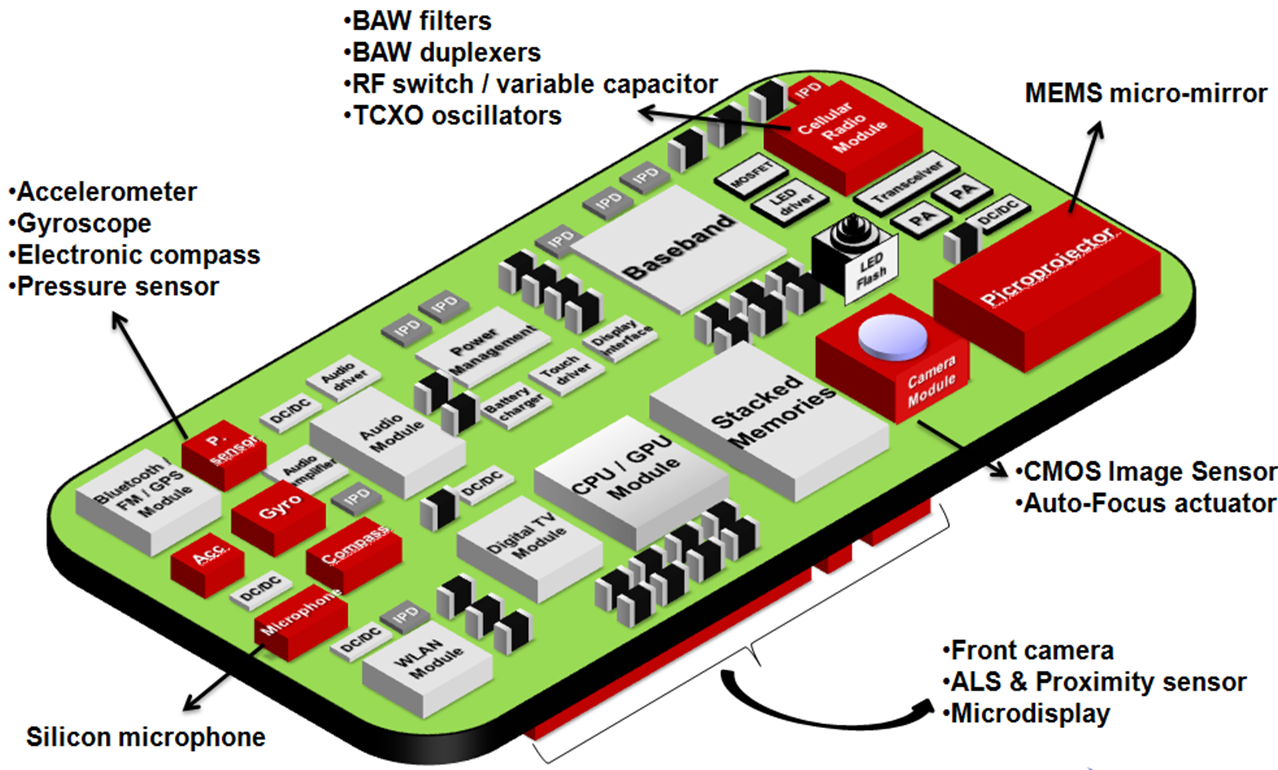
\includegraphics[scale=0.45]{Mobile_Device_Sensors.png}
	
	\btVFill
}

\section{\sectiontitleII}
% Section II - Frame I:
\frame{  \small
\frametitle{\sectiontitleII}


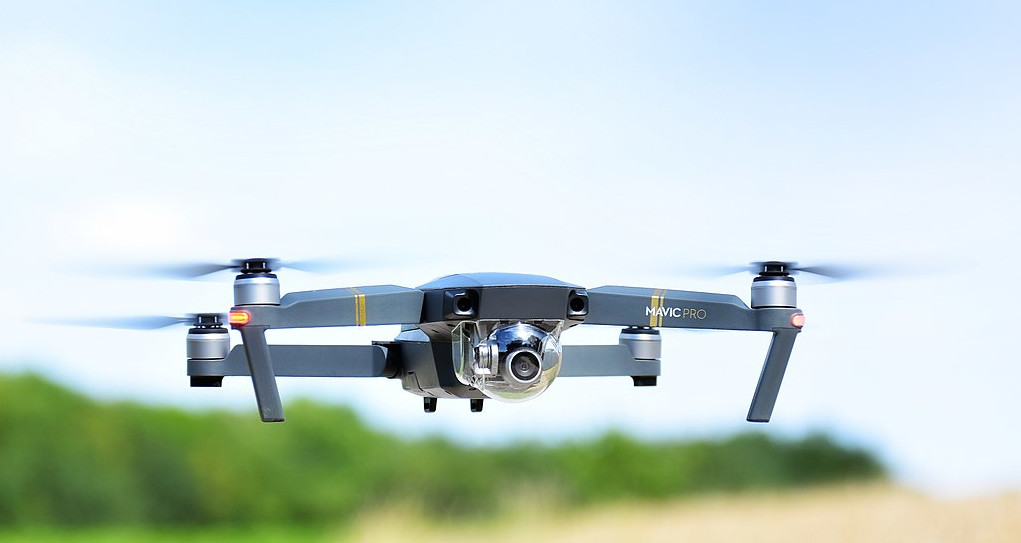
\includegraphics[scale=0.2]{Flying_DJI_Mavic_Pro_cropped.jpg}
	
	{\textbf Actvitity:} Group Brainstorming
	List three sensors that are found on a high performance quadcopter or drone.
	\begin{itemize}
		\item
		\item
		\item
	\end{itemize} 

 \btVFill



}

\section{\sectiontitleIII}

% Section III - Frame I:
\frame{  \small
\frametitle{\sectiontitleIII}

	An accelerometer is a tool that measures proper acceleration, which is the acceleration of a body in its own instantaneous frame.

	Applications:
	\begin{itemize}
		\item Navigation Systems - Robotics - Aircraft - Missiles
		\item Personal Devices - Phones - Tablets
		\item Others:
	\end{itemize}                                
 
    \btVFill
}

% Section III - Frame II:
\frame{  \small
\frametitle{\sectiontitleIII}
 	Thought Exercise: How do we measure acceleration? \vspace{10mm}\\                      
 	

 	{\textbf Actvitity:} Group Brainstorming \\
	Explain one method for measuring acceleration of a body.


    \btVFill

}

% Section III - Frame III:
\frame{  \small
\frametitle{\sectiontitleIII}
 	
	Mechanical Accelerometers Consist of a damped mass spring system and a sensing device.
	

 	Types of accelerometers:

 	\begin{itemize}
 		
 		\item Seismometer or Seismograph

 		\item piezoelectric - charge in material resulting from mechanical stress

 		\item piezoresistive - change in resistance resulting from mechanical stress

 		\item capacitive 

 	\end{itemize}

 
    \btVFill

}

% Section III - Frame II:
\frame{  \small
\frametitle{\sectiontitleIII}
 	piezoelectric accelerometer                                
 
 	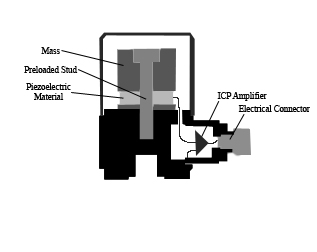
\includegraphics[scale=3.5]{PiezoAccel.jpg} 
 	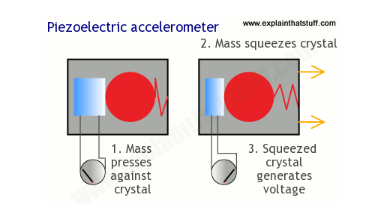
\includegraphics[scale=.55]{Piezoelectric.png}
    \btVFill

}

% Section III - Frame II:
\frame{  \small
\frametitle{\sectiontitleIII}
 	capacitive accelerometer                                
 
 	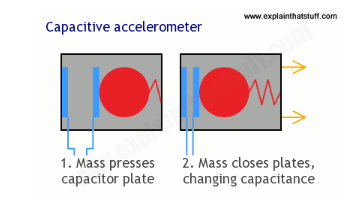
\includegraphics[scale=.55]{Capacitance.png}
    \btVFill

}



\section{\sectiontitleIV}

% Section IV - Frame I:
\frame{  \small
\frametitle{\sectiontitleIV}

	{\bf Thought Exercise:} How do we measure {\BL motion}?        
	
		\begin{itemize}
		
			\item What variable or quantity is used to describe motion?                         
			\begin{itemize}
				\item
				\item
				\item	
			\end{itemize} \vspace{5mm}
			\item What type of sensor is used to measure this?
			\begin{itemize}
				\item
				\item
				\item	
			\end{itemize}	

		\end{itemize}
	
	\btVFill


}

% Section IV - Frame II:
\frame{  \small
\frametitle{\sectiontitleIV}

	\begin{itemize}
	\item What applications require this type of sensor?
	\begin{itemize}
		\item \vspace{5mm}
		\item \vspace{5mm}
		\item \vspace{5mm}	
	\end{itemize}
\end{itemize}

\btVFill
}

%\section{\sectiontitleIV}

% Section V - Frame I:
\frame{  \small
	\frametitle{\sectiontitleIV}
	
	{\bf Thought Exercise:} How do we measure {\PR orientation}?        
	
	\begin{itemize}
		
		\item What variable or quantity is used to describe {\PR orientation}?                         
		\begin{itemize}
			\item
			\item
			\item	
		\end{itemize} \vspace{5mm}
		\item What type of sensor is used to measure this?
		\begin{itemize}
			\item
			\item
			\item	
		\end{itemize}	
		
	\end{itemize}
	
	\btVFill
	
	
}

% Section V - Frame II:
\frame{  \small
	\frametitle{\sectiontitleIV}
	
	\begin{itemize}
		\item What applications require this type of sensor?
		\begin{itemize}
			\item \vspace{5mm}
			\item \vspace{5mm}
			\item \vspace{5mm}	
		\end{itemize}
	\end{itemize}
	
	\btVFill
}

\end{document}

